\chapter{Implementación Game of Life}

%\section{}
% análisis
% Graficación
% Tabla rubrica

El programa se implementó en JavaScript que se muestra gráficamente en un canvas sobre un documento HTML, el código fuente está disponible en este enlace:
 \href{https://github.com/QApolo/CS/tree/master/03_Conway}{\textbf{Ver código y reporte}}
 \\\\
 Además, al ser un programa orientado web decidí lanzarla alojada gratuitamente por los servidores de Github,  por lo que es posible  acceder a ella y probar su funcionamiento, Enlace: \\ \href{https://qapolo.github.io/03_Conway/index.html}{\textbf{Aplicación Web}}
 
La rutina principal del código se puede ver abajo, donde es posible notar una pequeña optimización para no copiar todos los estados para la siguiente iteración, el array states de la linea 10 tiene como objetivo almacenar temporalmente únicamente aquellas células que presentan algún cambio en la matriz, lo que hace que la complejidad en memoria pase de \textbf{$O(w*h)$} a \textbf{$O(Y)$}  y que en promedio llega a ser menor que lineal, siendo $Y$ el número máximo de cambios en una iteración y $w$ y $h$ lo ancho y alto de la cuadricula.\\\\
\definecolor{mygray}{rgb}{0.66,0.66,0.66}

\lstset{backgroundcolor=\color{mygray}}
\lstinputlisting[language=Java, firstline = 82, lastline=149]{../game.js}
Al abrir el programa inmediatamente aparecen campos para darle una configuración al sistema, como se muestra en la Figura \ref{fig:menu}
\begin{figure}[h]
	\centering
	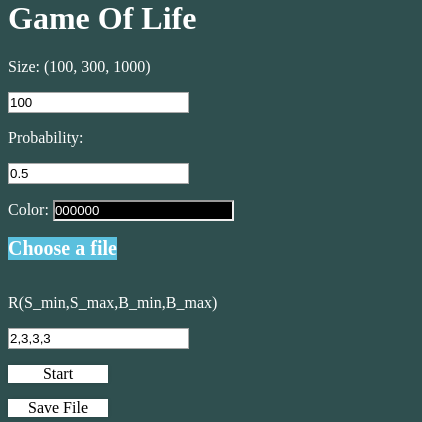
\includegraphics[width=0.7\textwidth]{capitulo2/images/menu.png}
	\caption{Parámetros del programa}
	\label{fig:menu}
\end{figure}
\newpage
\begin{itemize}
	\item \textbf{Size:} Se puede ingresar un tamaño desde 10, a 1000 denotando el tamaño cuadrado de la cuadricula.
	\item \textbf{Probability:} Es un valor entre 0 y 1 que indica la cantidad de unos en porcentaje iniciales de la cuadricula.
	\item \textbf{Color:} Al hacer click se mostrará una paleta de colores, con la que se podrá manipular en todo momento el color de los objetos en la cuadrícula.
	\item \textbf{Choose a File:} Al iniciar un programa podemos cargar un archivo de configuración cuya estructura se describe en la siguiente sección.
	\item \textbf{Start:} Una vez elegida una configuración podremos dar click a 'Start' y ver el comportamiento de la cuadrícula.
	\item \textbf{Save File} Podremos descargar un archivo de configuración en todo momento y posteriormente podremos cargarlo en otra instancia.
	\item \textbf{R(S\_min,S\_max,B\_min,B\_max):} Permite configurar la regla de evolución, con los valores ingresados separados por coma.
\end{itemize}

La cuadricula se muestra en la parte inferior al menú de configuración:
\begin{figure}[h]
	\centering
	
\includegraphics[width=0.5\textwidth]{capitulo2/images/01_grid.png}
	\caption{Cuadricula inicial con 50\% de células vivas.}
	\label{fig:01_grid}
\end{figure}

\newpage
La Figura \ref{fig:03_grid} muestra una selección de color que se ve reflejada en la cuadricula.
\begin{figure}[h]
	\centering
	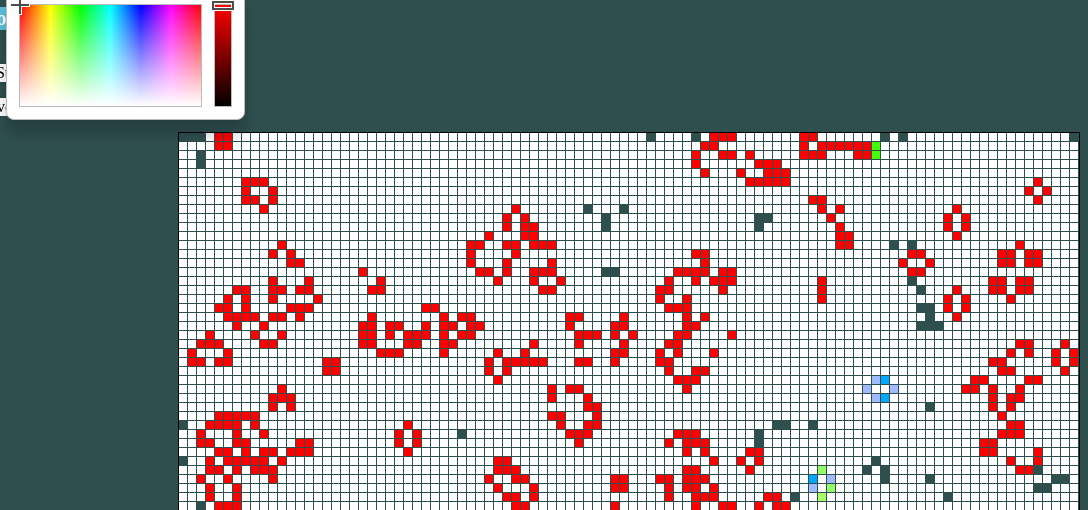
\includegraphics[width=0.6\textwidth]{capitulo2/images/03_grid.png}
	\caption{Cuadrícula con cambio de color instantáneo}
	\label{fig:03_grid}
\end{figure}
\newpage
También es posible dibujar nuestra propia configuración inicial con el puntero del ratón mientras se presiona la tecla \textbf{shift}.

\begin{figure}[h]
	\centering
	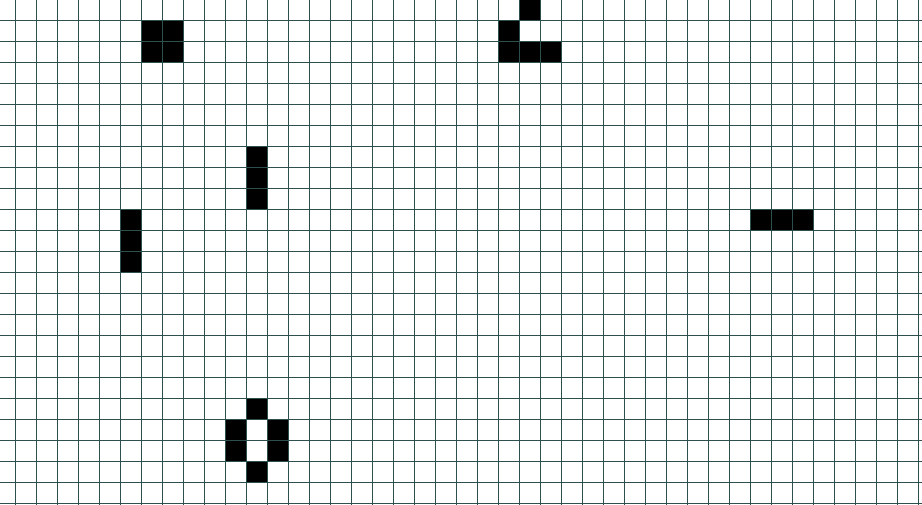
\includegraphics[width=0.6\textwidth]{capitulo2/images/03_plot.png}
	\caption{Patrones insertados manualmente}
	\label{fig:03_plot}
\end{figure}
Podemos apreciar que hay 3 Oscillator, 1 block,  1 Glider y 1 Beehive en la parte inferior, por lo que al darle iniciar podremos ver su rastro por la cuadricula.
\begin{figure}[h]
	\centering
	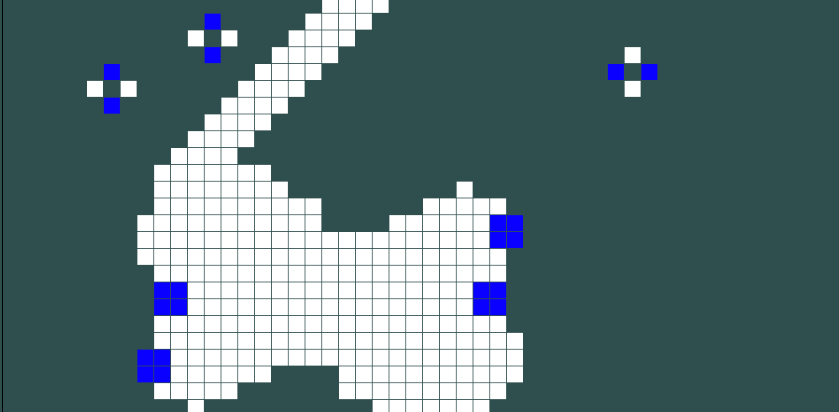
\includegraphics[width=0.6\textwidth]{capitulo2/images/04_plot.png}
	\caption{Rastro de los objetos, el glider colisiona con un oscillator y forma 4 blocks.}
	\label{fig:04_plot}
\end{figure}
\section{Archivo de configuración}
El archivo de configuración se compone de 4 partes, separadas por un salto de linea, la primera especifíca el tamaño de la cuadricula, siguiendo con el ejemplo anterior, 50x50.

La siguiente linea hace que la configuración del archivo tenga dos posibilidades (0 o 1):

\subsection{Con una nueva distribución de Células vivas}
Si el primer valor es 1, indica que la cuadricula se va a llenar nuevamente con la proporción especificada en el segundo valor siendo un flotante entre 0 y 1 y omitiendo la lectura de la matriz que representa a la cuadricula.
\subsection{Conservando la matriz que representa a la cuadricula}
Si el primer valor es 0, indica que se va a seguir con la matriz existente en el archivo, por lo que omitirá el valor de proporción y leerá la matriz para cargarla en el programa:
\lstset{backgroundcolor=\color{mygray}}
\lstinputlisting[ firstline = 1, lastline=3]{../configuration.txt}

La siguiente linea representa las unidades de tiempo discretas que vivirá el programa, para este caso en la linea 3 podemos ver que es de 100000 unidades.
\\\\
La matriz viene a continuación con valores de 0 y 1, el valor 0 indica una célula muerta y el valor 1, una célula viva, como se ve a continuación representando un segmento del ejemplo anterior donde se aprecia el block, el glider y los 3 oscillators, dos verticales y uno horizontal.
\lstset{backgroundcolor=\color{mygray}}
\lstinputlisting[ firstline = 4, lastline=20]{../configuration.txt}

\section{Gráfica}
El número de células vivas por generación se grafica en la parte inferior de la cuadrícula, el eje horizontal representa a las generaciones, mientras que el eje vertical la cantidad de células vivas en cada generación. 
\\\\
A continuación se muestra un ejemplo de 300x300 con un 50\% de células vivas:

\begin{figure}[h]
	\centering
	
\includegraphics[width=0.6\textwidth]{capitulo2/images/grid_plot.png}
	\caption{Rastro de los objetos, el glider colisiona con un oscillator y forma 4 blocks.}
	\label{fig:plotGrid}
\end{figure}

\begin{figure}[h]
	\centering
	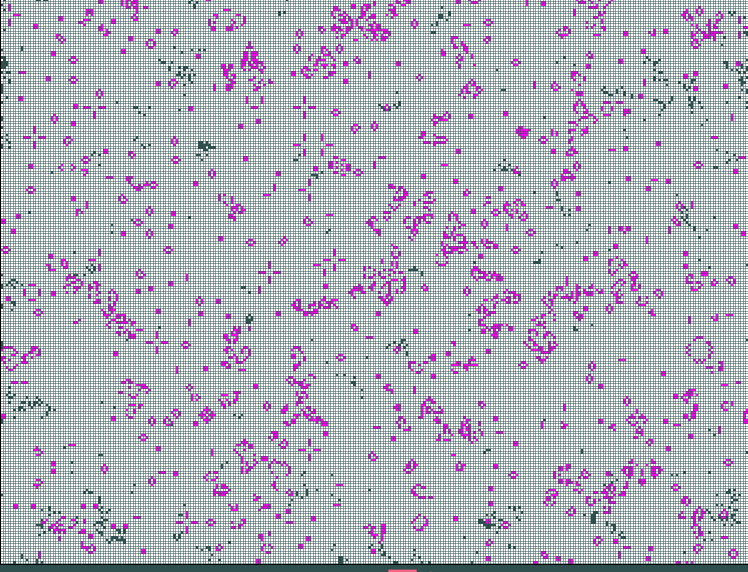
\includegraphics[width=0.6\textwidth]{capitulo2/images/300grid.png}
	\caption{Cuadricula de 300x300.}
	\label{fig:grid300}
\end{figure}
\newpage
La gráfica de células vivas muestra un comportamiento repentino decreciente al inicio.
\begin{figure}[h]
	\centering
	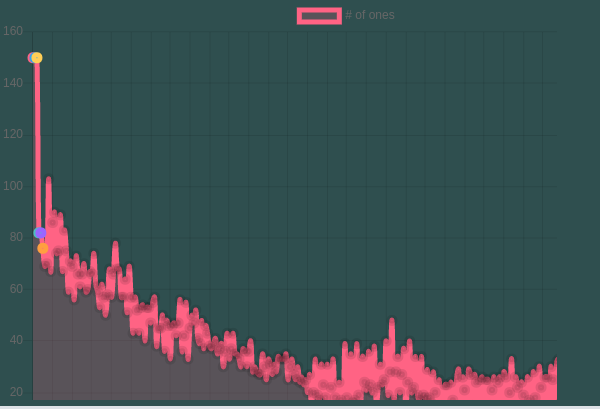
\includegraphics[width=0.6\textwidth]{capitulo2/images/300plot.png}
	\caption{Gráfica de cuadricula de 300x300.}
	\label{fig:plot300}
\end{figure}
\newpage
Donde después de cierto tiempo muestra signos de estabilizarse para mostrar una monotonía constante.

\begin{figure}[h]
	\centering
	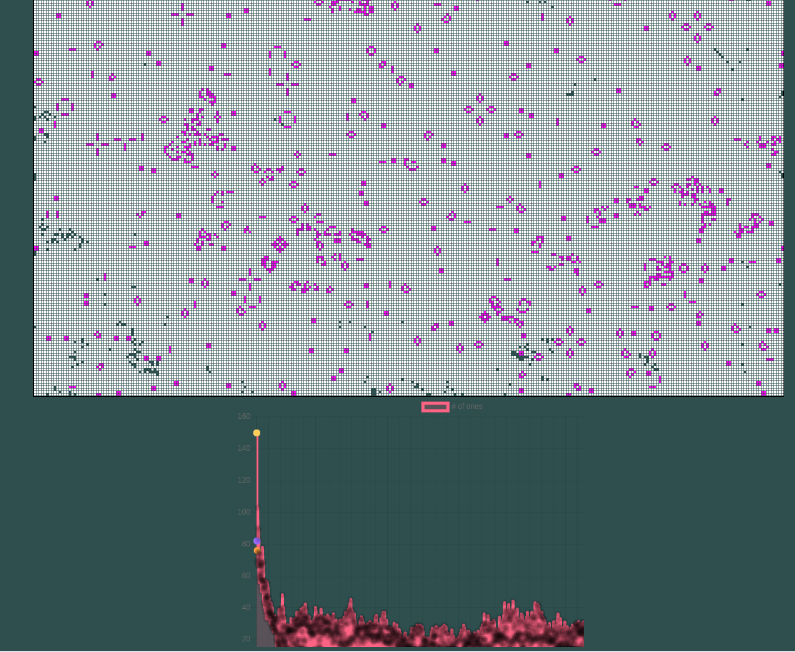
\includegraphics[width=0.6\textwidth]{capitulo2/images/300plotgrid2.png}
	\caption{Cuadrícula y su gráfica}
	\label{fig:grid300_2}
\end{figure}
\newpage
Al ser de 300x300 el poder lograr ver esa monotonía constante en la gráfica requiere de muchas generaciones o unidades de tiempo, sin embargo en una cuadricula de 100x100 es más rápido ver este comportamiento como se muestra en la Figura \ref{fig:time_grid} y en la Figura \ref{fig:time_plot}

\begin{figure}[h]
	\centering
	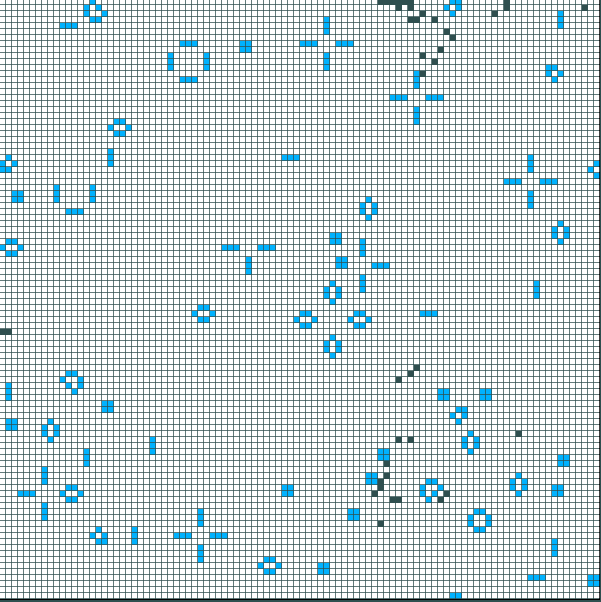
\includegraphics[width=0.6\textwidth]{capitulo2/images/time_grid.png}
	\caption{Cuadricula de 100x100 con patrones constantes}
	\label{fig:time_grid}
\end{figure}
Podemos ver como esta tiende a una función constante y que se puede ver debido a que los patrones constan de oscillators y blocks que mantienen el número de células vivas muy constante por periodos.
\begin{figure}[h]
	\centering
	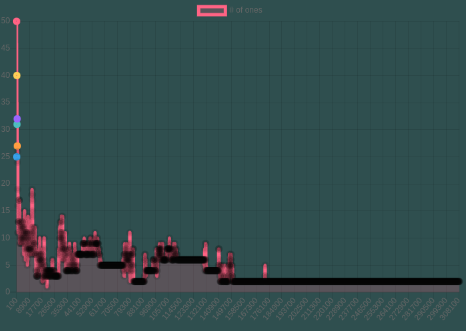
\includegraphics[width=0.6\textwidth]{capitulo2/images/time_plot.png}
	\caption{Gráfica de la cuadricula de 100x100}
	\label{fig:time_plot}
\end{figure}
\newpage
\section{Regla de evolución}
Por defecto el programa carga la regla \textbf{R(2, 3, 3, 3)}, que es la propuesta originalmente, sin embargo es posible modificar estos valores y observar el comportamiento del autómata.
\\\\
Algo interesante es ver el caso en el que $S_{min} = S_{max} = B_{min} = B_{max}$, podría pensarse que esta generalidad da lugar a un resultado similar, sin embargo 
al hacer pruebas se puede concluir que no es generalizable del todo, ya que si $S_{min} = S_{max} = B_{min} = B_{max} = i$ con $i \in \{1,2\}$ hay una constancia periódica del número de células vivas, mientras que para $S_{min} = S_{max} = B_{min} = B_{max} \geq 3$ prácticamente todas las células vivas mueren con gran aceleración: 
\newpage
\subsection{R(2,2,2,2)}
El comportamiento de la regla cuando los parámetros son igual a 2, tiene también un comportamiento similar cuando son igual a 1, en la Figura \ref{fig:R2222}.
\begin{figure}[h]
	\centering
	\subfigure[]{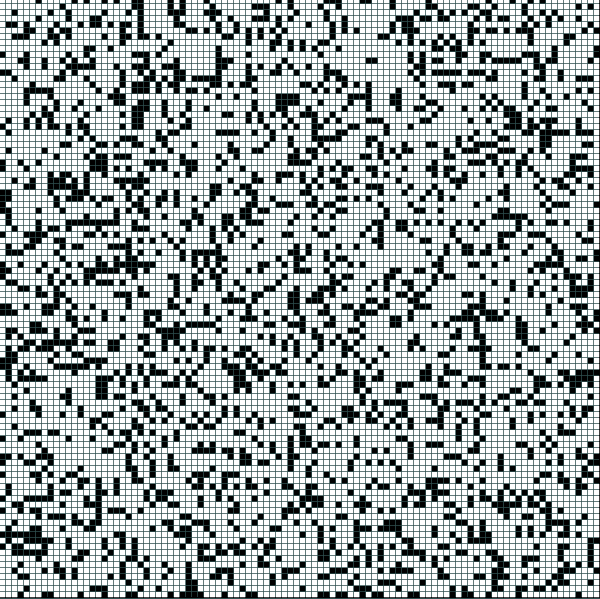
\includegraphics[width=0.3\textwidth]{capitulo2/images/R2222.png}} 
	\subfigure[]{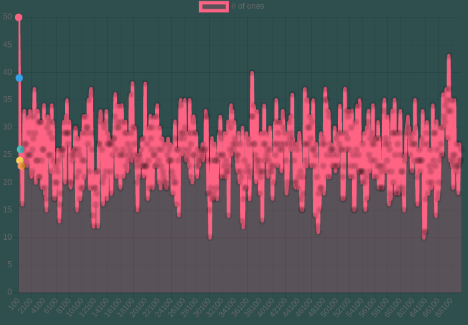
\includegraphics[width=0.3\textwidth]{capitulo2/images/R_plot2222.png}}
	\caption{(a) Cuadrícula con regla R(2,2,2,2) (b) Gráfica de células vivas.}
	\label{fig:R2222}
\end{figure}
\newpage
\subsection{R(3,3,3,3)}
Para la regla con valores iguales mayores que 2, el patrón hace que haya una tasa muy alta de células muertas en cada generación, dejando en la mayoría de los casos un tablero con todas las células muertas.
\begin{figure}[h]
	\centering
	\subfigure[]{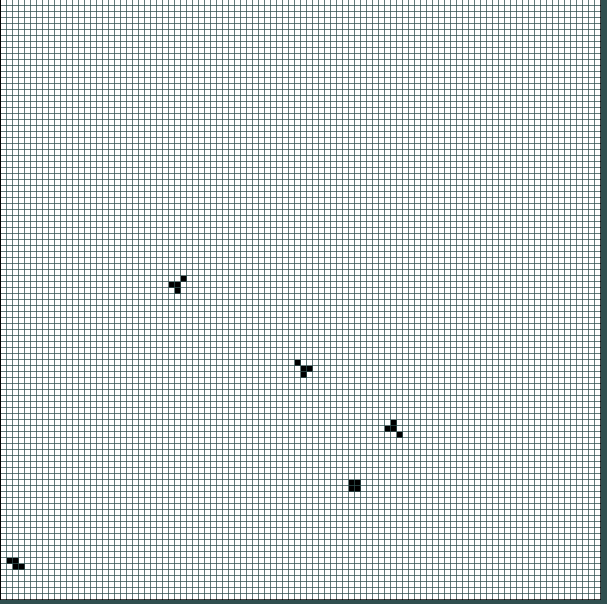
\includegraphics[width=0.4\textwidth]{capitulo2/images/R3333.png}} 
	\subfigure[]{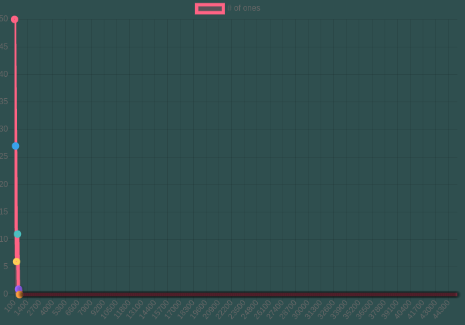
\includegraphics[width=0.4\textwidth]{capitulo2/images/R_plot3333.png}}
	\caption{(a) Cuadrícula con regla R(3,3,3,3) (b) Gráfica de células vivas.}
	\label{fig:R3333}
\end{figure}
\newpage
\subsection{R(1,2,3,4)}
Esta regla produce patrones constantes en cuanto a periocidad, lo que genera gráficas relativamente constantes en cuanto a periodo.
\begin{figure}[h]
	\centering
	\subfigure[]{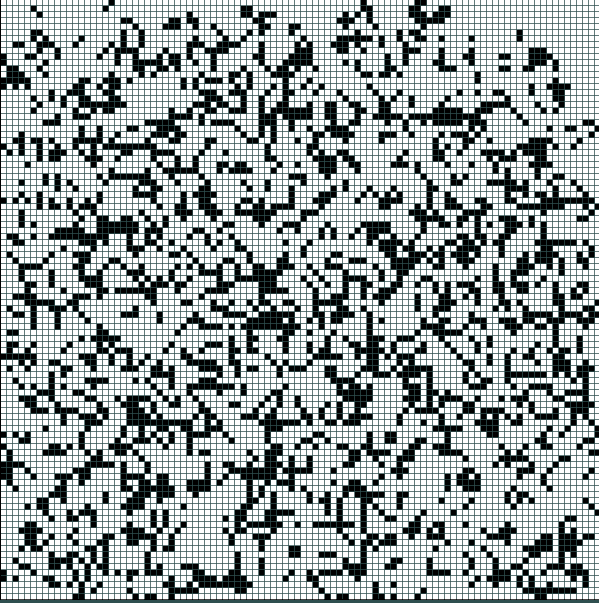
\includegraphics[width=0.4\textwidth]{capitulo2/images/R1234.png}} 
	\subfigure[]{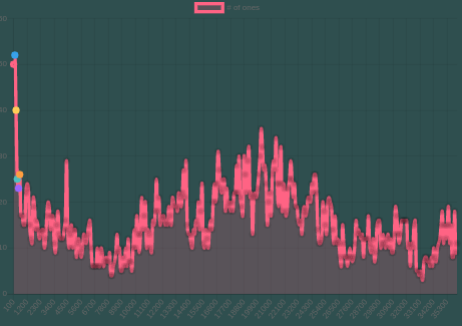
\includegraphics[width=0.4\textwidth]{capitulo2/images/R_plot1234.png}}
	\caption{(a) Cuadrícula con regla R(1,2,3,4) (b) Gráfica de células vivas.}
	\label{fig:R1234}
\end{figure}
\newpage
\subsection{R(2,4,6,8)}
En el caso de esta regla, después de pocas generaciones se puede ver una constancia en cada una de las generaciones siguientes, produciendo en su mayoría oscillators de periodo simple y patrones tipo Still Life que se ve reflejada en la gráfica.
\begin{figure}[h]
	\centering
	\subfigure[]{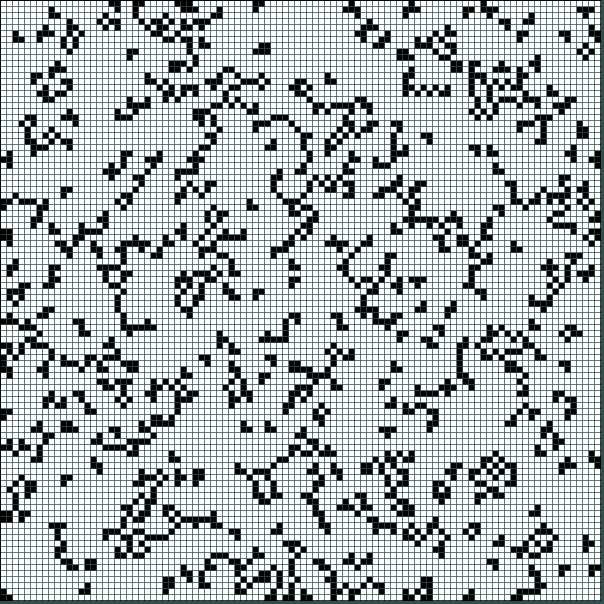
\includegraphics[width=0.4\textwidth]{capitulo2/images/R2468.png}} 
	\subfigure[]{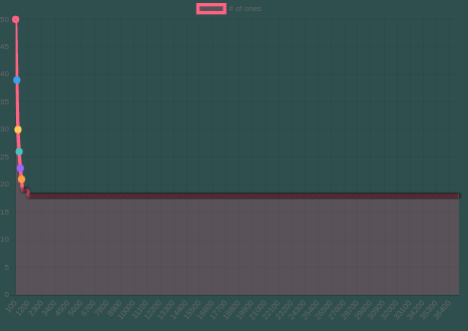
\includegraphics[width=0.4\textwidth]{capitulo2/images/R_plot2468.png}}
	\caption{(a) Cuadrícula con regla R(2,4,6,8) (b) Gráfica de células vivas.}
	\label{fig:R2468}
\end{figure}

\newpage

\subsection{R(2,3,3,4)}
Esta regla de evolución aunque muy parecida a la R(12,3,4), parece que agrega volumen a los patrones, produciendo un buen efecto visual, también se debe mencionar que mantiene en términos numéricos una cantidad de células vivas y muertas aunque variable parece garantizar que el autómata conservará su densidad impidiendo que los objetos Still Life duren por mucho tiempo.
\begin{figure}[h]
	\centering
	\subfigure[]{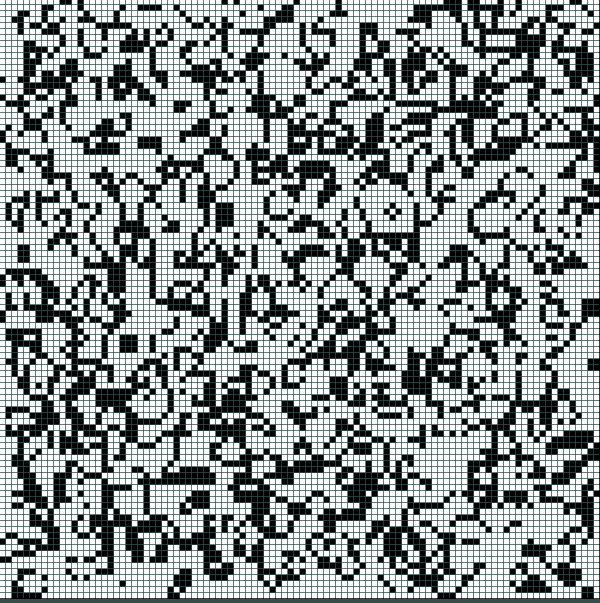
\includegraphics[width=0.4\textwidth]{capitulo2/images/R2334.png}} 
	\subfigure[]{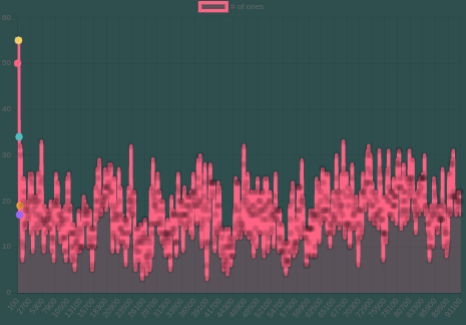
\includegraphics[width=0.4\textwidth]{capitulo2/images/R_plot2334.png}}
	\caption{(a) Cuadrícula con regla R(2,3,3,4) (b) Gráfica de células vivas.}
	\label{fig:R2334}
\end{figure}

\newpage


El programa cumple con las características propuesas que se enlistan a continuación:

\begin{tabularx}{1.0\textwidth} { 
		| >{\raggedright\arraybackslash}X 
		| >{\centering\arraybackslash}X 
		| >{\raggedleft\arraybackslash}X | }
	
	\hline
	No.  & Característica \\
	\hline
	1  &Evaluar espacios de 300x300, 500x500 y máximo de 1000x1000 células  \\
	\hline
	2 & Animación en dos dimensiones   \\
	\hline
	3   &  Poder cambiar los colores del estado  \\
	\hline
	4   & Poder inicializar el espacio de evoluciones con diferentes densidades  \\
	\hline
	5  &   Poder editar el espacio de evoluciones para dibujar configuraciones particulares\\
	\hline
	6 & Poder salvar y levantar archivos con configuraciones en específico \\
	\hline
	7 & Graficar el número de unos de cada generación\\
	8 & Editar la regla de evolución $R(S\_min,S\_max,B\_min,B\_max)$\\
	\hline
\end{tabularx}\\
	Características del programa del juego de la vida.